\section{Planning}
My planning can be found in \autoref{fig:planning}. The indicated time needed for the programming tasks is indicative since this will be largely determined by how many issues will be encountered along the way. Testing and validation of the code will be done iteratively, which is why it is scheduled for almost the whole duration of the thesis. Near the end of the project, when as much code is offloaded as possible, more comprehensive performance assessments will be done (also scheduled under "Testing and validation"). I will be writing the report parallel to the programming and research, I plan to devote about a third of my time to writing. 

\begin{figure}[H]
    \centering
    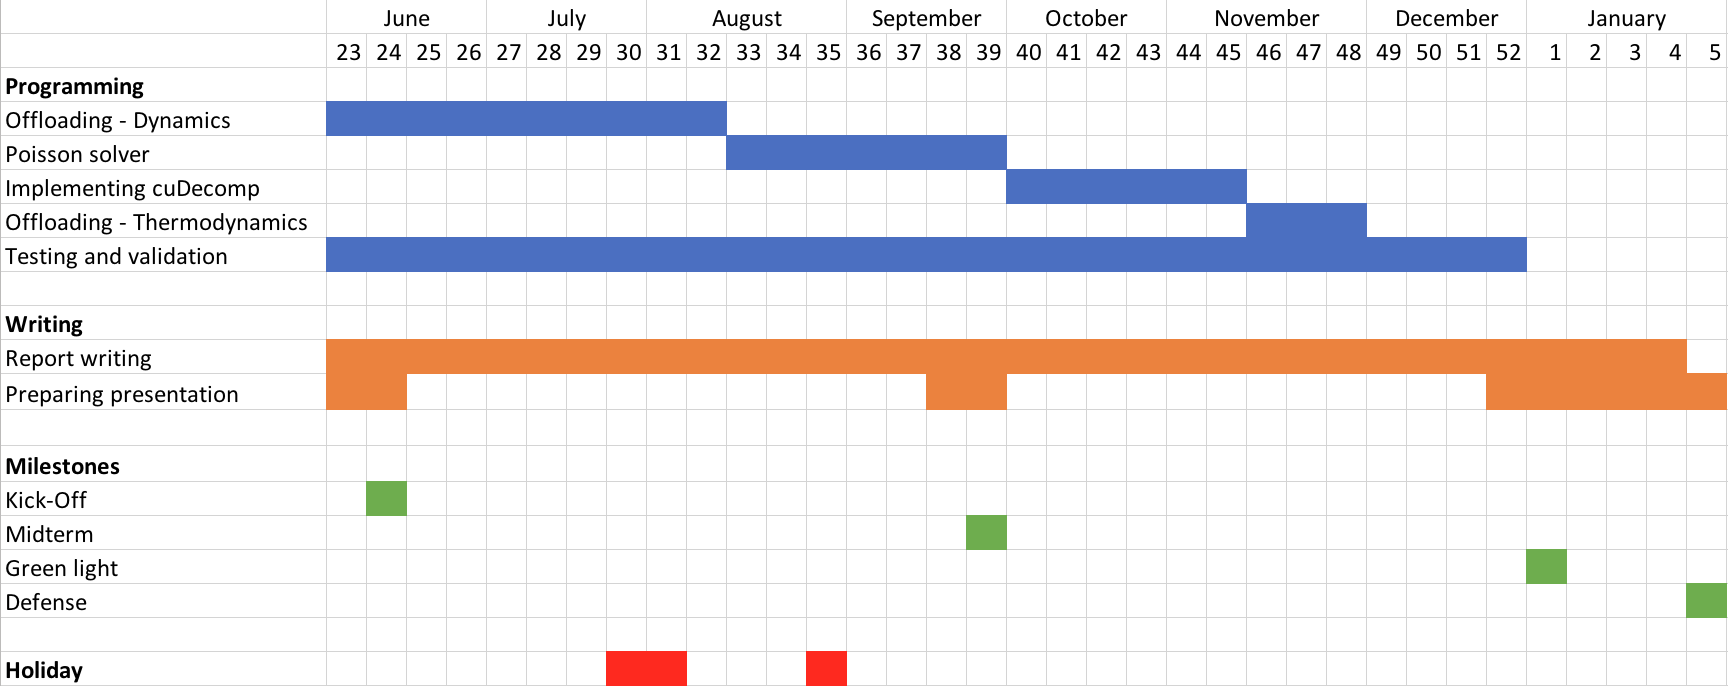
\includegraphics[width=\textwidth]{doc/images/planning.png}
    \caption{Weekly planning}
    \label{fig:planning}
\end{figure}